\documentclass[12pt,oneside]{report}
\usepackage{graphicx}
\usepackage{epstopdf}
\usepackage{fancyhdr}
\usepackage{tabularx}
\usepackage{mathrsfs,amsmath}
\usepackage[table]{xcolor}
%some decoration for black cell tabular
\newcommand\BlackCell[1]{%
  \multicolumn{1}{c}{\cellcolor{black}\textcolor{white}{#1}}
}
\usepackage{tikz}
\newcommand*\circled[1]{\tikz[baseline=(char.base)]{
            \node[shape=circle,draw,thick,inner sep=0pt,minimum size=17pt] (char) {#1};}}
%creating fancy header and footer
\fancyhf{}
\lhead{Medical Imaging}
\chead{Homework 2}
\rhead{P.H.An-9651}
\cfoot{\thepage}
%font=default,size 12pt
%Configure page layout: a4, margin 0.79in, onesided, indent 0.5in
\paperwidth=8.27in
\paperheight=11.69in
\voffset=-0.21in
\hoffset=-0.21in
\oddsidemargin=0in
\evensidemargin=0in
\topmargin=-23pt
\headheight=12pt
\headsep=25pt
\marginparsep=0in
\marginparwidth=0in
\footskip=30pt
\marginparpush=0in
\textwidth=6.69in
\textheight=9.61in
%indent of a first line of new paragraphc is 0.5in to use \indent or \par
\parindent=0.5in
%set distance btw lines
\baselineskip=0pt
%set disctance btw pars
\parskip=0pt
%create a listing environment for arranging text
%tree level 1: {\textbullet}{0in}{0in}{\parindent}
%tree level 2: dependent :D
\newenvironment{tree}[6]{
\begin{list}{#1}{\parskip=0in \topsep=#5 \itemsep=#6 \parsep=0in \partopsep=0in \leftmargin=#2 \rightmargin=#3 \itemindent=#4 \listparindent=\itemindent}
}{\end{list}}
%creat a small section document :D
\newenvironment{ssection}[7]{
\framebox{\textbf{#1}} \textbf{#2}
\begin{tree}{#3}{#4}{#5}{\parindent}{#6}{#7}
}{\end{tree}}
%fix other errors manually if needed: line break, etc.
\begin{document} %SINUSOIDAL STEADY-STATE ANALYSIS
\thispagestyle{plain}
\pagestyle{fancy}
\noindent
\begin{tabular}{c}
\BlackCell{\parbox{\textwidth}{}}\\
\BlackCell{\parbox{\textwidth}{\centerline{{\Large \textbf{\emph{Homework 2}}}}}}\\
\BlackCell{\parbox{\textwidth}{}}\\
\end{tabular}
\begin{flushright}
\large \textit{Phan Hoang An - 9651}
\end{flushright}
\ \\
\begin{ssection}{Problem 4.1}{}{}{0in}{0in}{7pt}{0pt}
\item It is \textbf{\textit{true}} that an FID signal lasts as long as the transverse magnetization. This is a test. Hi. I need real time.
\end{ssection}
\ \\
\begin{ssection}{Problem 4.2}{}{}{0in}{0in}{7pt}{0pt}
\item For a spin system with $N$ spectral components at their corresponding individual frequencies, the spectral density function $\rho(\omega)$
is a combination of $N$ delta functions of frequencies:
\begin{center}
$\rho(\omega)=\displaystyle\sum_{k=1}^{N}M^{0}_{z,k}\delta(\omega-\omega_{k})$
\end{center}
In addition, an FID signal resulting from an $\alpha$ pulse is mathematically presented by:
\begin{center}
$S(t)=\displaystyle\sin\alpha\int_{-\infty}^{\infty}\rho(\omega)e^{-t/T_2(\omega)}e^{-j\omega t}d\omega$
\end{center}
Thus, an FID signal with $N$ spectral components can be derived as follows:
\begin{center}
\begin{tabular}{l}
\hphantom{$\Rightarrow\ $}$ S(t)=\displaystyle\sin\alpha\int_{-\infty}^{\infty}\sum_{k=1}^{N}M^{0}_{z,k}\delta(\omega-\omega_{k})
e^{-t/T_2(\omega)}e^{-j\omega t}d\omega$\\
$\Rightarrow S(t)=\displaystyle\sin\alpha\sum_{k=1}^{N}\left(M^{0}_{z,k}\int_{-\infty}^{\infty}
\delta(\omega-\omega_{k})e^{-t/T_2(\omega)}e^{-j\omega t}d\omega\right)$
\end{tabular}
\end{center}
For any function $f(x)$ defined within $[a,b]$, we consider the following characteristic
\begin{center}
$\displaystyle\int_{a}^{b}\delta(x-x_0)f(x)dx=f(x_0),\ \forall x_0 \in [a,b]$
\end{center}
Hence, with any $k \in [1,N]$, we easily see that
\begin{center}
$\displaystyle\int_{-\infty}^{\infty}\delta(\omega-\omega_{k})e^{-t/T_2(\omega)}e^{-j\omega t}d\omega=e^{-t/T_2(\omega_k)}e^{-j\omega_k t}$
\end{center}
Therefore, we finally obtain the expression of a FID with $N$ spectral components,
\begin{center}
$S(t)=\displaystyle\sin\alpha\sum_{k=1}^{N}M^{0}_{z,k}e^{-t/T_2(\omega_k)}e^{-j\omega_k t}$
\end{center}
\end{ssection}
\ \\
\begin{ssection}{Problem 4.11}{}{}{0in}{0in}{7pt}{0pt}
\item \circled{a} Let's denote $M_z^0$ as the bulk magnetization at thermal equilibrium. So, we have,
\begin{center}
$\begin{cases}
\mbox{the process } \vec{M}_{rot}(0_{-})\xrightarrow{90_{x'}^o}\vec{M}_{rot}(0_{+})\xrightarrow{90_{y'}^o}\vec{M}_{rot}(0_{++})\\
\mbox{the pre-pulse condition }\vec{M}_{rot}(0_{-})=[0,0,M_z^0]^T
\end{cases}$
\end{center}
\par \hspace*{0.5\parindent}\textbullet Calculation of $\vec{M}_{rot}$ after $90_{x'}^o$-pulse: $\vec{M}_{rot}(0_{+})=R_{x'}(90^o)\vec{M}_{rot}(0_{-})$
\begin{center}
%\begin{tabular}{l}
$\Rightarrow\vec{M}_{rot}(0_{+})=
\begin{bmatrix} 
1 & 0 & 0\\ 
0 & \cos 90^o & \sin 90^o\\
0 & -\sin 90^o & \cos 90^o 
\end{bmatrix}
\begin{bmatrix} 
0\\
0\\
M_z^0
\end{bmatrix}
=\begin{bmatrix} 
0\\
M_z^0\\
0
\end{bmatrix}
$\\
%\end{tabular}
\end{center}
\par \hspace*{0.5\parindent}\textbullet Calculation of $\vec{M}_{rot}$ after $90_{y'}^o$-pulse: $\vec{M}_{rot}(0_{++})=R_{y'}(90^o)\vec{M}_{rot}(0_{+})$
\begin{center}
%\begin{tabular}{l}
$\Rightarrow\vec{M}_{rot}(0_{++})=
\begin{bmatrix} 
\cos 90^o & 0 & -\sin 90^o\\
0 & 1 & 0\\
\sin 90^o & 0 & \cos 90^o 
\end{bmatrix}
\begin{bmatrix}
0\\
M_z^0\\
0
\end{bmatrix}
=\begin{bmatrix} 
0\\
M_z^0\\
0
\end{bmatrix}
$\\
%\end{tabular}
\end{center}
\par \hspace*{0.5\parindent}\textbullet Sketch the bulk magnetization $\vec{M}_{rot}(t)$ after the two pulses
\begin{center}
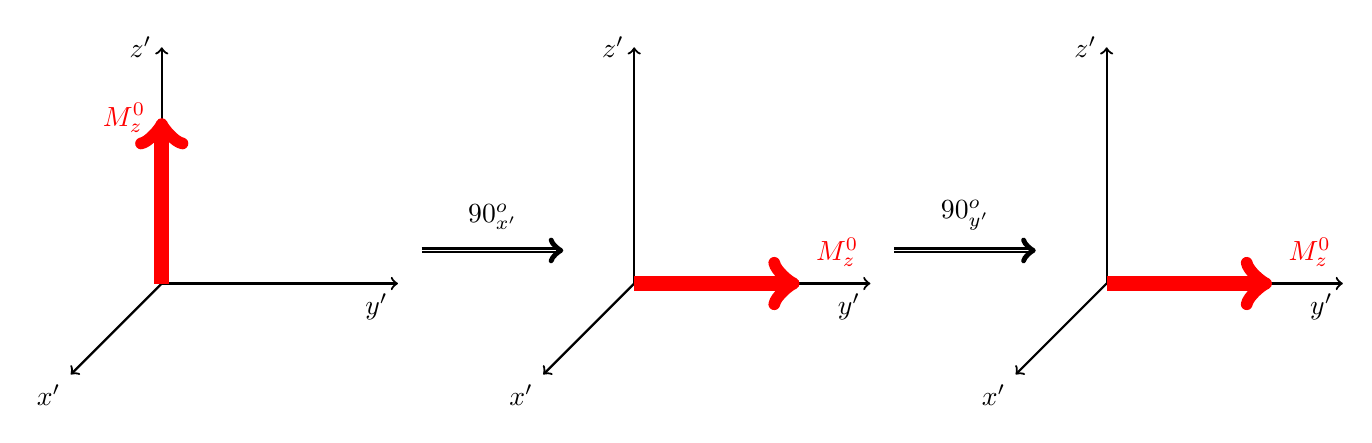
\begin{tikzpicture}[scale=3,cm={-1,-1,1,0,(0,0)},x=3.85mm,z=-1cm]
\draw[thick,->] (0,0,0) -- (1,0,0) node[anchor=north east]{$x'$};
\draw[thick,->] (0,0,0) -- (0,1,0) node[anchor=north east]{$y'$};
\draw[thick,->] (0,0,0) -- (0,0,1) node[anchor=east]{$z'$};
\coordinate (A) at (0,0,0);
\coordinate (B) at (0,0,0.7);
\draw[red, line width=5.3pt, ->] (A) -- (B) node[anchor=east]{$M_z^0$};
\draw[thick, double,->] (0,1.1,0.14) -- node[label=88:$90_{x'}^o$] {} (0,1.7,0.14);
\begin{scope}[shift={(0,2)}]
\draw[thick,->] (0,0,0) -- (1,0,0) node[anchor=north east]{$x'$};
\draw[thick,->] (0,0,0) -- (0,1,0) node[anchor=north east]{$y'$};
\draw[thick,->] (0,0,0) -- (0,0,1) node[anchor=east]{$z'$};
\draw[red, line width=5.3pt, ->] (0,0,0) -- (0,0.7,0) node[anchor=south west]{$M_z^0$};
\draw[thick, double,->] (0,1.1,0.14) -- node[label=88:$90_{y'}^o$] {} (0,1.7,0.14);
\end{scope}
\begin{scope}[shift={(0,4)}]
\draw[thick,->] (0,0,0) -- (1,0,0) node[anchor=north east]{$x'$};
\draw[thick,->] (0,0,0) -- (0,1,0) node[anchor=north east]{$y'$};
\draw[thick,->] (0,0,0) -- (0,0,1) node[anchor=east]{$z'$};
\draw[red, line width=5.3pt, ->] (0,0,0) -- (0,0.7,0) node[anchor=south west]{$M_z^0$};
\end{scope}
\end{tikzpicture}
\end{center}
\item \circled{b} From the sketch, because the signal has only one single spectral component, it is obvious that the FID signals $S_1(t)$ and $S_2(t)$ generated by the two pulses are \emph{\textbf{the same}}.
\end{ssection}
\ \\
\begin{ssection}{Problem 4.12 a}{}{}{0in}{0in}{7pt}{0pt}
\item Let's denote the two given processes as follows:
\begin{center}
$\begin{cases}
\mbox{Process 1: } \vec{M}_{rot}(0_{-})\xrightarrow{90_{x'}^o}\vec{M}_{rot}(\tau_{-})\xrightarrow{\tau}
\vec{M}_{rot}(\tau_{+})\xrightarrow{180_{y'}^o}\vec{M}_{1}\\
\mbox{Process 2: } \vec{M}_{rot}(0_{-})\xrightarrow{90_{x'}^o}\vec{M}_{rot}(\tau_{-})\xrightarrow{\tau}
\vec{M}_{rot}(\tau_{+})\xrightarrow{180_{x'}^o}\vec{M}_{2}
\end{cases}$
\end{center}
\par The sketch of the bulk magnetization vector from the time point $\tau_{+}$ onwards,
\begin{center}
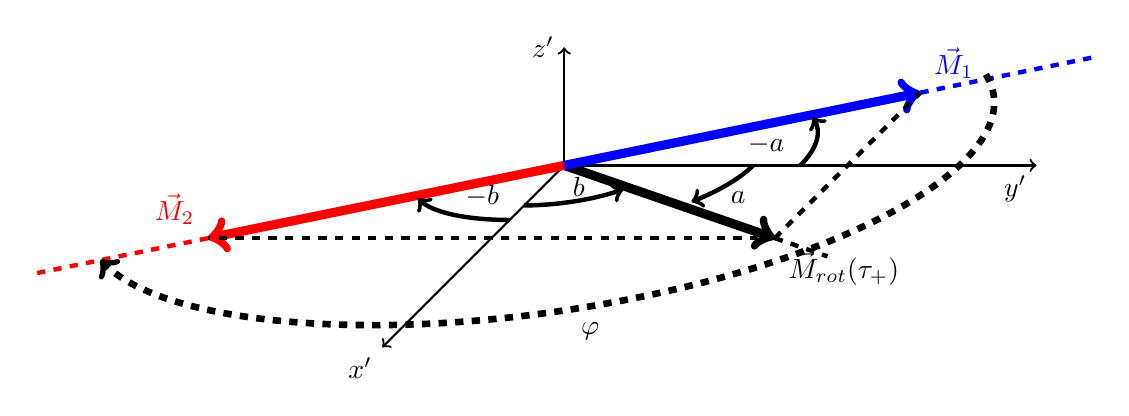
\begin{tikzpicture}[scale=3,cm={-1,-1,1,0,(0,0)},x=2*3.85mm,y=2cm,z=-0.5cm]
\draw[thick,->] (0,0,0) -- (1,0,0) node[anchor=north east]{$x'$};
\draw[thick,->] (0,0,0) -- (0,1,0) node[anchor=north east]{$y'$};
\draw[thick,->] (0,0,0) -- (0,0,1) node[anchor=east]{$z'$};
\draw[line width=3.3pt, ->] (0,0,0) -- (0.4,0.6,0) node[anchor=north west]{$\vec{M}_{rot}(\tau_{+})$};
\draw[ultra thick, ->] (0,0.4) arc (90:60:0.4);
\node[] at (68:0.47) {$a$};
\draw[ultra thick, ->] (0.22,0) arc (0:53:0.22);
\node[] at (33:0.14) {$b$};
\draw[blue, line width=3.3pt, ->] (0,0,0) -- (-0.4,0.6,0) node[anchor=south west]{$\vec{M}_{1}$};
\draw[ultra thick, ->] (0,0.5) arc (90:122:0.5);
\node[] at (107:0.4) {$-a$};
\draw [dashed, ultra thick] (0.4,0.6) -- (-0.4,0.6);
\draw[red, line width=3.3pt, ->] (0,0,0) -- (0.4,-0.6,0) node[anchor=south east]{$\vec{M}_{2}$};
\draw[ultra thick, ->] (0.3,0) arc (0:-53:0.3);
\node[] at (-33:0.2) {$-b$};
\draw [dashed, ultra thick] (0.4,0.6) -- (0.4,-0.6);
\draw [red,dashed, ultra thick] (0.4,-0.6) -- (0.6,-0.9);
\draw [dashed, ultra thick] (0.4,0.6) -- (0.5,0.75);
\draw [blue,dashed, ultra thick] (-0.4,0.6) -- (-0.6,0.9);
\draw[dashed, line width=2.4pt, ->] (-0.5,0.7) arc (122:-53:0.9);
\node[] at (24:1) {$\varphi$};
\end{tikzpicture}
\end{center}
\par It can be seen that the two echo signals resulted from $\vec{M}_{1}$ and $\vec{M}_{2}$ should be equal in their magnitude, and have $180^o$ phase difference. To illustrate, lets consider some angle coordination as in the sketch, then $\varphi=-(-a)+a-b+(-b)=2(a-b)=2(-\pi/2)=-\pi$ or $180^o$.
\end{ssection}
\newpage
\noindent
\begin{ssection}{Problem 4.19}{}{}{0in}{0in}{7pt}{5pt}
\item \circled{a} $B_z(x,y,z)=3-2x\Rightarrow\vec{\nabla} B_z=\displaystyle\frac{\partial(3-2x)}{\partial x}\vec{i}
+\frac{\partial(3-2x)}{\partial y}\vec{j}+\frac{\partial(3-2x)}{\partial z}\vec{z}=-2\vec{i}$
\par 
\hspace*{0.5\parindent} $\Rightarrow$ A linear $x$-gradient field with $G_x=-2$.
\item \circled{b} $B_z(x,y,z)=3-2x+x^2\Rightarrow\vec{\nabla} B_z=\displaystyle\frac{\partial(3-2x+x^2)}{\partial x}\vec{i}
+\frac{\partial(3-2x+x^2)}{\partial y}\vec{j}+\frac{\partial(3-2x+x^2)}{\partial z}\vec{z}$\\
\hphantom{$B_z(x,y,z)=3-2x ab\qquad\qquad\quad$} $\Rightarrow \vec{\nabla} B_z=(-2+2x)\vec{i} \Rightarrow$ Not a linear gradient field.
\item \circled{c} $B_z(x,y,z)=5-x-y-z\Rightarrow\vec{\nabla} B_z=-\vec{i}-\vec{j}-\vec{k} \Rightarrow$ A linear gradient field.
\end{ssection}
\ \\
\begin{ssection}{Problem 5.1}{}{}{0in}{0in}{7pt}{0pt}
\item It is \textbf{\emph{false}} that selection of an envelope function for an RF pulse has nothing to do with the $\vec{B}_0$ field strength. Because the sharp of RF envelope function together with the inhomogeneity of the $\vec{B}_0$ field will affect the number of selective spectral components (or the scaling interval of equally two-sided rectangular function in frequency domain) in the transverse magnetization vector (the solution of Bloch equation in which both $\vec{B}_0\mbox{ and }\vec{B}_1$ participate) as well as in the selection accuracy of expected parts of an object.
\end{ssection}
\ \\
\begin{ssection}{Problem 5.4}{}{}{0in}{0in}{7pt}{0pt}
\item In the slice-selective excitation, the \textbf{\emph{cross-talk}} artifacts means the unexpected excitation of spins in the neighboring slices to some varying degrees, which is due to the truncation of RF-pulse (spatially support-limited time-domain signal impacts on entire frequency-domain).
\end{ssection}
\end{document}